%!TEX root = ../../thesis.tex

Before discussing the software architecture in section~\ref{sec:software_architecture}, sections \ref{sec:rich_text_approaches} through \ref{sec:las_before_software_architecture} will discuss the apporaches, principles and goals for implementing this library without HTML editing APIs.

\section{Approaches for enabling rich-text editing}
\label{sec:rich_text_approaches}

%When not using HTML editing APIs, the components and the bahavior of native text inputs must be imitated. There are various approaches to this.

%\paragraph{Overlaying an element in editing mode} One way to 

This section will discuss the options to implement rich-text editing without relying (entirely) on HTML editing APIs and discuss the advantages and disadvantages of each method. % Diese Art zu schreiben sollte der Style der Arbeit sein.

\paragraph{Native input elements} Native text inputs are hard-wired to plain-text editing. No major browser offers an API for formatting. There is also no option to write HTML to an input and have it display it as rich-text. \texttt{input} fields and \texttt{textarea} elements will simply display the HTML as source code. Rich-text can only be implemented as an editable part of the website.

\paragraph{Image elements} In February 2015, Flipboard Inc. demonstrated an unprecedented technique to achieve fluid full-screen animations with 60 frames per second on their mobile website\footnote{\url{http://engineering.flipboard.com/2015/02/mobile-web/}, last checked on 07/24/2015}. Instead of using the DOM to display their contents, the entire website was rendered to a \texttt{canvas} element. When a user swiped over the website the canvas element was rerendered, essentially imitating the browser's rendering engine. \texttt{canvas} elements allow rendering rich-text too. A rich-text editor can be implemented using this technique. This however has two major downsides. On the one hand it would require implementing a text-rendering engine. The \texttt{canvas} API is only capable of displaying unlayouted text with specifically set line breaks. On the other hand, making the editor accessible to other developers would be much more complex since the text only exists in an internal representaion inside the editor and would not be exposed as DOM component on the website.

An approach related to rendering the text on a \texttt{canvas} element is to render the text inside a Scalable Vector Graphic (SVG). In contrast to \texttt{canvas} elements, SVGs contain DOM nodes that can be accesed from the outside. However this has no benefit over using HTML DOM nodes with the downside that SVG too has no native implementation for controlling the text flow.

\paragraph{Enabling editing mode without using its API} One way to enable editing but avoiding many bugs and browser inonstistencies, is to enable the editing mode on an element, but avoid using \texttt{execCommand} to format the text. The latter could be implemented using the DOM core APIs. This would provide the user with all basic editing functions, i.e. a caret, text input, mouse interaction and clipboard capabilites. All of this would be taken care of by the browser.

This sem-radical approach would solve the problem of buggy and inconsistent \texttt{execCommand} implementations but not the problems that arise with different browser behavior on the user's text input---for instance when entering a line break. If the markup is customly generated with JavaScript, the input may break elements or simply get stuck. This was one of the reasons why Google decided to abandon editing APIs entirely\footnote{\url{http://googledrive.blogspot.fr/2010/05/whats-different-about-new-google-docs.html}, last checked on 07/21/2015}. It could be the source to many bugs, have the development of the library be dependent on browser development and ultimatively restrict the editors capabilites.

\paragraph{Native text input imitation} The only other option to allow the user to change the text on a website is by manually fetching the user's input and manipulating the DOM with JavaScript. However, this does not suffice to provide the experience of a text input. The following components, common to text editing, must also be accounted for:
% These components will be discussed hereinafter.

%, major browsers offer no way to place a caret

% Only native text input components and elements in editing mode
% ''ACE'' and ''CodeMirror'' demonstrate an effective way to imitate a text input. 

 %''ACE'' and ''CodeMirror'' demonstrate it is possible to imitate a text input by composing various DOM ele
\paragraph{Caret} The most obvious part is probably the text caret. Even if a user types on his or her keyboard, a caret must be seen on the screen to know where the input will be inserted. The caret also needs to be responsive to the user's interaction. In particular, the user must be able to click anywhere in the editable text and use the arrow keys to move it (possibly using modifier keys, which's behaviour even depends on the operating system used).

\paragraph{Selection} Just like the caret, the user must be able to draw a text selection using his or her mouse and change the selection using shift and the arrow keys. Most systems allow double clicks to select words and sometimes tripple clicks to select entire paragraphs. Other systems, for example OS X, allow holding the option key to draw are rectengular text selection, independent of line breaks.

\paragraph{Context menu} The context menu is different in text inputs from other elements on a website. Most importantly, it offers an option to paste text, that is only available in native text inputs or elements in editing mode.

\paragraph{Keyboard shortcuts} Text inputs usually allow keyboard shortcuts to format the text and to perform clipboard operations. Formatting the text is possible through DOM manipulation, pasting text however natively only works on text inputs or elements in editing mode. % is a challenge, since browsers do not offer arbitrary access to the clipboard for security reasons.

\paragraph{Undo / Redo} Undo and redo are common functions of text processing and it may be frustrating to users if they were missing.

\paragraph{Behaviour} Rich-text editors (usually) share a certain behaviour on user input. When writing a bulleted list, pressing the enter key usually creates another bulleting point instead of inserting a new line. Pressing enter inside a heading will insert a new line. However pressing enter when the caret is located at the end of a heading commonly creates a new text paragraph just after that heading. Other rules that need to be considered will be discussed in section [implementation].

\paragraph{Imitating native components} These components are natively available for text inputs across all browsers. Switching an element to editing mode enables these components too. That means a user can click in a text to place a caret and move it with the keyboard's arrow keys. He or she can copy and paste text. The browser offers a native context menu that allows pasting on input elements as well as on element in editing mode. All major browsers implement a behaviour for the user' input that is common for rich-text editing (as described above).

When not using editing APIs, all of this must be implemented with JavaScript. This requires a lot of trickery and many components must be imitated to make it \textit{seem} there is an input field, where there is none. The user must be convinced he or she is using a native input and must not notice he or she is not.

\begin{figure}[!htb]
\centering
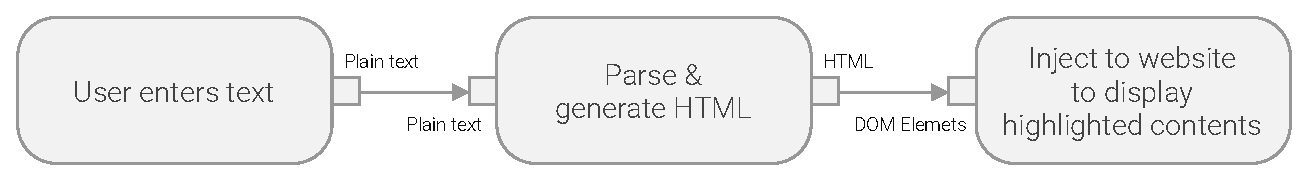
\includegraphics[scale=.7]{images/ace-codemirror-uml.eps}
\caption{Rendering of highlighted source code in Ace and CodeMirror}
\label{fig:ace_rendering_uml}
\end{figure}


Web-based code editors like ''Ace'' and ''CodeMirror'' demonstrate that this is possible. They display syntax-highlighted source code editable by the user. The user seemingly writes inside the highlighted text and is also presented with a caret as well as the above mentioned components. In reality, the content inside the editor that a user sees is a regular part of the DOM---non-editable text, colored and formatted using HTML and CSS. When the user enters text, the input will be read with JavaScript. Based on the input Ace and CodeMirror generate HTML and add it to the editors contents, to show a properly syntax-highlighted representation (see figure~\ref{fig:ace_rendering_uml}). A \texttt{div} element that is styled to look like a caret is shown and moved with the user's keyboard and mouse input. The user's text input will be inserted at the according text offset. Amongst others, Ace and CodeMirror use other elements like \texttt{div}s to display a text selection and a \texttt{textarea} to fetch keyboard inputs, to recreate the behavior and capabilites of a native text input. Google's document editor uses similar techniques too.

%In reality, the user's input will be read with JavaScript and the code he or she sees is HTML generated based on this input to display syntax-highlighted text. Other components, like the caret and even the selection \texttt{div} elements, styled and positioned to mimick their native counterparts. 

%All this creates the illusion of a native text input.

%Many of the techniques to mimick a native text input like this can be found in web-based code editors like ''ACE'' or ''CodeMirror''.

Using tricks and \textit{faking} elements or behavior is common in web front end development. This applies to JavaScript as well as to CSS. For instance, long before CSS3 has been developed, techniques (often called ''hacks'') have been discussed on how to implement rounded corners without actual browser support. Only years later, this has become a standard. This not only enables features long before the creators of browsers implement them, this \textit{feedback} by the community of web developers also influences future standards. Encorporating feedback is a core philisophy of the WHATWG, the creators of HTML5.

Hacks are a necessity for an editor like this. The following sections will discuss each part of the editor and describe ideas, techniques and hacks that can be used for an effective implementation. In prior, we will discuss goals and principles that these techniques should be oriented towards as well as restrictions of browsers these techniqes must adapt to. % worst sentence ever

\section{Usage of HTML elements}

Ace, CodeMirror and Google's document editor shre similar concepts for imitating a native text input. For the caret, each of the editors create a \texttt{div} element, style it to make it look like a caret and move it when the user clicks in the text or uses his or her arrow keys. Each editor uses \texttt{div} elements to display a text selection, styled to imitate the user's operating system's native selections. %In fact, there is hardly no alternative way

The concept to use HTML elements for the visible components of text editing is inevitable. Anything that can be seen on a website must exist in the DOM. The only deviation to this approach would be to resort a \texttt{canvas} element, as discussed above. The apporach to use HTML elements will be used for the implementation of this editor.

% Google, unlike Ace and CodeMirror displays a custom context menu. 

\section{Interaction with browser APIs}

Interaction with the browser must be well chosen. In some cases browser interaction can cause bugs and slow down performance while in some cases it can increase performance. The library should conform these rules:

\begin{enumerate} 
\item Minimize interaction with the DOM
\item Minimize interaction with unstable APIs
\item Use browser APIs if it improves performance or structure
\end{enumerate}

DOM operations can trigger a browser reflow\footnote{\url{https://developers.google.com/speed/articles/reflow}, last checked on 07/19/2015} which slows down the browser's performance. For this reason DOM operations should be avoided where possible.

Some APIs like the browser's \texttt{Range} or \texttt{Selection} interface are useful but known to be unstable. Libraries like Rangy try to tackle this by shimming parts of the interfaces. This requires complex methods and it is hard to account for possibly unknown bugs in the browsers' APIs. Ultimately this will also affect the library's file size. Instead of trying to fix native APIs, only as little as possible should be used. Instead of using possibly unstable APIs, pure JavaScript implementations should be used. Possibly unstable native APIs should only be used when it is inevitable.

Avoiding DOM operations and unstable APIs leads to a software architecture where the biggest part remains in its own business logic. Anything that can be implemented in pure JavaScript and does not cost performance or memory \textit{should} be implemented in pure JavaScript using own methods and data structues.

Facebook defined a similar goal for the user interface library React. React implements virtual DOM, an internal represenation of the actual DOM on which all operations should be performed, which in return does as little manipulation to the actual DOM as needed, to maximize performance. While the focus of this goal for this library is not solely performance, this part of it. However, there can be situations in which (even unstable) native browser methods may be faster than a JavaScript implementation. The text flow for instance should be left to the browser. There can also be cases in which a pure JavaScript implementation would be much more complex and would be at the expense of having a simple code structure. It must be decided in each particular case to use native and possible unstable APIs or a pure JavaScript implementation.

\section{Conformity with HTML Editing APIs}

The library should be capable of any method that HTML editing APIs implement. However the API can differ to improve they way it will be worked with. Improving means it should be more explicit in what it does. The \texttt{bold} command of \texttt{execCommand} will manipulate the DOM to format text bold. It does not state in what how. Simple etc, what I have stated at Disadvantages of offering user interface components.

\section{Markup} 

Our editor should be a good citizen in this ecosystem. That means we ought to produce HTML that’s easy to read and understand. And on the flip side, we need to be aware that our editor has to deal with pasted content that can’t possibly be created in our editor. https://medium.com/medium-eng/why-contenteditable-is-terrible-122d8a40e480

Also FirePad and Google generate unusable markup. we're gonna generate semantic markup, simple and clean.

%\section{Partially using HTML editing APIs}

%That would be one way \textbf{note: try to show all the options for implementation for WeWu}


\section{Stability and performance}

\paragraph{Cache} For traversing the text, for example when the caret moves, the text will need to be measured. All measurements can be stored to a cache to only perform the same measurement operations once. On the other hand, the library should be a ''good citizen'' on a website, which means it should be as unobtrusive and leave the developers as much freedom as possible. The library will essentially modify parts of the DOM that act as the editor's contents. It should be agnostic to the editor's contents at all times to give other developers the freedom to change the contents in any way needed without breaking the editor. A cache must account for external changes. The DOM3 Events specification\footnote{\url{http://www.w3.org/TR/DOM-Level-3-Events/}, last checked on 07/21/2015} offers \texttt{MutationObserver}s to check for DOM changes. This feature is not supported by Internet Explorer version 10 or less\footnote{\url{http://caniuse.com/\#search=mutation}, last checked on 07/21/2015}. Internet Explorer 9 and 10 offer an implementation for \texttt{MutationEvent}s\footnote{\url{http://help.dottoro.com/ljfvvdnm.php\#additionalEvents }, last checked on 07/21/2015}. The W3C states that ''The MutationEvent interface [...] has not yet been completely and interoperably implemented across user agents. In addition, there have been critiques that the interface, as designed, introduces a performance and implementation challenge.''\footnote{\url{http://www.w3.org/TR/DOM-Level-3-Events/\#legacy-mutationevent-events}, last checked on 07/21/2015}. Apart from that, the benefits of a cache may not signifcantly increase the library's performance. The actions that can be supported by a cache, most importantly moving the caret in the text, are not very complex and do not noticably afflict the CPU. Implementing an editor that is stateless in regards of its contents can also improve stability.

% dom operations could also be cached

\section{Disadvantages of offering user interface components}

Most rich-text editors are implemented and distributed as user interface components. That means instead of only providing a library that offers methods to format the selected text and leaving the implementation of the user interface to the respective developer, most libraries are shipped as input fields with a default editor interface that is, at best, customizable.

This can be unfitting for many situations. The user interface of an editor highly depends on the software it will be integrated in. Within the software the interface may even vary depending on the specific purpose within it. For instance, a content management system may require an edtitor with a menubar offering many controls while a comment form on a blog requires only very little controls. Medium.com uses an interface that only shows controls when the user selects text and has no menubar at all. Assuming there are many implementations of editors, it seems, choosing between editors is often just a choice of the desired ui. Customizing a ui can be just as complex as writing a ui from scratch. The latter affords to add HTML elememts and call JavaScript methods. In a worst case styling the elements can be just as much effort. That is why the library ''Type'' will be implemented and offered as a software library, rather than an editor and a user interface component.

It can be much more fitting for developers to include a library that handles all text-input and -formatting operations while only providing a powerful API, leaving the ui to the developer. The API must be \textit{well-designed}. That means it must be simple, effective and fit the developers' needs. The methods it offers should be simple in the sense that they conceal possibly complex tasks with understandable high-level concepts. They should be effective and fit the developers' needs in the sense that the API should be designed so that any requirements should be matched with as little effort as possible. The API should create a workflow for developers that allows them to do what they want to do and is as easy to use as possible. jQuery is an example of encorporating an API conforming these principles.

\section{iFrame}

iFrame hat vor und nachteile. mit meiner library kann es jeder so machen, wie er/sie es will, weil es nur ne library ist.


\section{API Design}
\label{sec:las_before_software_architecture}

Allgemeine Überlegungen wie man ein Framework gestaltet (siehe ''Freiheit für Programmierer'', gute Arbeitsweise)
Ursprünglich API und Codestruktur an window.execCommand orientiert, das ist aber doof.
Bessere (weil präzisere) API mit mehr Möglichkeiten als der contentEditable scheiss
für Programmierer und für 2 anwendungsfälle:
einen editor bauen
type mit plugins erweitern
für beides gibt es die passenden Funktionen, das eine einfach und schlau, das andere präzise
Deswegen werden auch alle Module, alle Klassen exponiert aber es gibt eine eigene API nach jQuery konzept
Type kommt mit bestimmten Kernmodulen die fuer Textbearbeitung essenziell sind. Aber an dieser Stelle laesst sich Type um weitere Module anhand einer KOnvention (erweitern des Type Objekts) erweitern.
Ursprünglich API und Codestruktur an window.execCommand orientiert, das ist aber doof.

\section{Software architecture}
\label{sec:software_architecture}

\paragraph{MVC}
Document model -> no
Ursprünglich MVC mäßig mit document im kern geplant 